\documentclass[11pt,openany]{book}
\usepackage[]{graphicx}\usepackage[]{color}
%% maxwidth is the original width if it is less than linewidth
%% otherwise use linewidth (to make sure the graphics do not exceed the margin)
\makeatletter
\def\maxwidth{ %
  \ifdim\Gin@nat@width>\linewidth
    \linewidth
  \else
    \Gin@nat@width
  \fi
}
\makeatother

\definecolor{fgcolor}{rgb}{0.345, 0.345, 0.345}
\newcommand{\hlnum}[1]{\textcolor[rgb]{0.686,0.059,0.569}{#1}}%
\newcommand{\hlstr}[1]{\textcolor[rgb]{0.192,0.494,0.8}{#1}}%
\newcommand{\hlcom}[1]{\textcolor[rgb]{0.678,0.584,0.686}{\textit{#1}}}%
\newcommand{\hlopt}[1]{\textcolor[rgb]{0,0,0}{#1}}%
\newcommand{\hlstd}[1]{\textcolor[rgb]{0.345,0.345,0.345}{#1}}%
\newcommand{\hlkwa}[1]{\textcolor[rgb]{0.161,0.373,0.58}{\textbf{#1}}}%
\newcommand{\hlkwb}[1]{\textcolor[rgb]{0.69,0.353,0.396}{#1}}%
\newcommand{\hlkwc}[1]{\textcolor[rgb]{0.333,0.667,0.333}{#1}}%
\newcommand{\hlkwd}[1]{\textcolor[rgb]{0.737,0.353,0.396}{\textbf{#1}}}%
\let\hlipl\hlkwb

\usepackage{framed}
\makeatletter
\newenvironment{kframe}{%
 \def\at@end@of@kframe{}%
 \ifinner\ifhmode%
  \def\at@end@of@kframe{\end{minipage}}%
  \begin{minipage}{\columnwidth}%
 \fi\fi%
 \def\FrameCommand##1{\hskip\@totalleftmargin \hskip-\fboxsep
 \colorbox{shadecolor}{##1}\hskip-\fboxsep
     % There is no \\@totalrightmargin, so:
     \hskip-\linewidth \hskip-\@totalleftmargin \hskip\columnwidth}%
 \MakeFramed {\advance\hsize-\width
   \@totalleftmargin\z@ \linewidth\hsize
   \@setminipage}}%
 {\par\unskip\endMakeFramed%
 \at@end@of@kframe}
\makeatother

\definecolor{shadecolor}{rgb}{.97, .97, .97}
\definecolor{messagecolor}{rgb}{0, 0, 0}
\definecolor{warningcolor}{rgb}{1, 0, 1}
\definecolor{errorcolor}{rgb}{1, 0, 0}
\newenvironment{knitrout}{}{} % an empty environment to be redefined in TeX

\usepackage{alltt}
\newcommand{\SweaveOpts}[1]{}  % do not interfere with LaTeX
\newcommand{\SweaveInput}[1]{} % because they are not real TeX commands
\newcommand{\Sexpr}[1]{}       % will only be parsed by R


\usepackage[utf8]{inputenc} 
\usepackage{amssymb, amsmath, amsthm}
\usepackage{fullpage}
\usepackage{setspace}
\usepackage{graphicx}
\usepackage{natbib}
\usepackage{rotating}
\usepackage{caption}
\usepackage{subcaption}
\usepackage{multirow}
\usepackage{booktabs}
\usepackage{dcolumn}
\usepackage[grey]{quotchap}
\usepackage{xcolor}
\usepackage[left=1in, top=1in, right=1.5in, bottom=1in, headsep=.5in]
{geometry}
\usepackage{fancyhdr, blindtext}
\usepackage{diagbox}
\usepackage{hyperref} 
\usepackage{placeins}
\renewenvironment{knitrout}{\begin{singlespace}}{\end{singlespace}}
\newcommand*{\mybox}[2]{\colorbox{#1!30}{\parbox{.98\linewidth}{#2}}}
\newcommand*{\befehl}[1]{\texttt{\textbackslash #1}} % Added by 


\fancyhf{}
\fancyhead[LE]{\slshape \rightmark} 
\fancyhead[RE]{\thepage}
\fancyhead[RO]{\slshape \leftmark} 
\fancyhead[LO]{\thepage}
\renewcommand{\headrulewidth}{0.4pt}
\pagestyle{fancy}
%% new command for greybox
\long\def\greybox#1{%
    \newbox\contentbox%
    \newbox\bkgdbox%
    \setbox\contentbox\hbox to \hsize{%
        \vtop{
            \kern\columnsep
            \hbox to \hsize{%
                \kern\columnsep%
                \advance\hsize by -2\columnsep%
                \setlength{\textwidth}{\hsize}%
                \vbox{
                    \parskip=\baselineskip
                    \parindent=0bp
                    #1
                }%
                \kern\columnsep%
            }%
            \kern\columnsep%
        }%
    }%
    \setbox\bkgdbox\vbox{
        \pdfliteral{0.85 0.85 0.85 rg}
        \hrule width  \wd\contentbox %
               height \ht\contentbox %
               depth  \dp\contentbox
        \pdfliteral{0 0 0 rg}
    }%
    \wd\bkgdbox=0bp%
    \vbox{\hbox to \hsize{\box\bkgdbox\box\contentbox}}%
    \vskip\baselineskip%
}
%% make greybox (grbox) a float
\usepackage{float}
\newfloat{grbox}{thp}{lop}[section]
\floatname{grbox}{Grey Box}



\begin{document}


\chapter{Exploring and Visualizing Data}



You have your plan, you carry out your plan by getting out and collecting your data, and then you put your data into a file.  You are excited to test your hypothesis so you immediately run your multiple regression analysis and look at your output.  You can do that (and probably will even if we advise against it), but what you need to do before you can start to make sense of that output is to look carefully at your data.  You will want to know things like ``how much spread do I have in my data" and ``do I have any outliers".  (If you have limited spread, you may discover that it is hard to explain variation in something that is nearly a constant and if you have an outlier, your statistics may be focused on trying to explain that one case.) 

In this chapter, we will identify the ways to characterize your data before you do serious analysis both to understand what you are doing statistically and to error-check.

\section{Characterizing Data}


What does it mean to characterize your data? First, it means knowing how many observations are contained in your data, and the distribution of those observations over the range of your variable(s). What kinds of measures (interval, ordinal, nominal) do you have, and what are the ranges of valid measures for each variable? How many cases of missing (no data) or mis-coded (measures that fall outside the valid range) do you have? What do the coded values represent? While seemingly trivial, checking and evaluating your data for these attributes can save you major headaches later. For example, missing values for an observation often get a special code -- say, ``-99" -- to distinguish them  from valid observations. If you neglect to treat these values properly, R (or any other statistics program) will treat that value as if it were valid and thereby turn your results into a royal hairball. We know of cases in which even seasoned quantitative scholars have made the embarrassing mistake of failing to properly handle missing values in their analyses. In at least one case, a published paper had to be retracted for this reason. So don't skimp on the most basic forms of data characterization!

The dataset used for purposes of illustration in this version of this text is taken from a survey of Oklahomans, conducted in 2016, by OU's Center for Risk and Crisis Management. The survey question wording and background will be provided in class. However, for purposes of this chapter, note that the measure of  \textbf{ideology} consists of a self-report of political ideology on a scale that ranges from 1 (strong liberal) to 7 (strong conservative); the measure of the \textbf{perceived risk of climate change} ranges from zero (no risk) to 10 (extreme risk). \textbf{Age} was measured in years. 

It is often useful to graph the variables in your data set to get a better idea of their distribution. In addition, we may want to compare the distribution of a variable to a theoretical distribution (typically a normal distribution). This can be accomplished in several ways, but we will show two here---a histogram and a density curve---and more will be discussed in later chapters. Here we examine the distribution of the variable measuring the perceived risk of climate change. 

A histogram creates intervals of equal length, called bins, and displays the frequency of observations in each of the bins. To produce a histogram in R simply use the geom_histogram command in the \texttt{ggplot2} package. Next, we  plot the density of the observed data along with a normal curve.  This can be done with the \texttt{geom_density} command in the \texttt{ggplot2} package. 

Note that the normal distribution overlay using the \texttt{stat_function} function for the \texttt{gccrsk} variable is based on the mean and standard deviation of the \textttt{age} variable. The results are shown in Figure \ref{fig:rsk_2}. As you can see, the \texttt{age} variable is not quite normally distributed.  The histogram illustrates that the majority of observations are contained in the upper half of the variable's range.  Moreover, the density curve indicates the the distribution if negatively skewed, and the peak of the distribution is higher on the \texttt{gccrsk} scale than that of the theoretical normal distribution.




\begin{knitrout}
\definecolor{shadecolor}{rgb}{0.969, 0.969, 0.969}\color{fgcolor}\begin{kframe}
\begin{alltt}
\hlkwd{ggplot}\hlstd{(ds,} \hlkwd{aes}\hlstd{(age))} \hlopt{+}
  \hlkwd{geom_density}\hlstd{()} \hlopt{+}
   \hlkwd{stat_function}\hlstd{(}\hlkwc{fun} \hlstd{= dnorm,} \hlkwc{args} \hlstd{=} \hlkwd{list}\hlstd{(}\hlkwc{mean} \hlstd{=} \hlkwd{mean}\hlstd{(ds}\hlopt{$}\hlstd{age,} \hlkwc{na.rm} \hlstd{= T),}
                                            \hlkwc{sd} \hlstd{=} \hlkwd{sd}\hlstd{(ds}\hlopt{$}\hlstd{age,} \hlkwc{na.rm} \hlstd{= T)),} \hlkwc{color} \hlstd{=} \hlstr{"red"}\hlstd{)}
\hlkwd{dev.off}\hlstd{()}
\end{alltt}
\end{kframe}
\end{knitrout}

\begin{figure}
        \centering
        \begin{subfigure}[b]{0.4\textwidth}
                \centering
                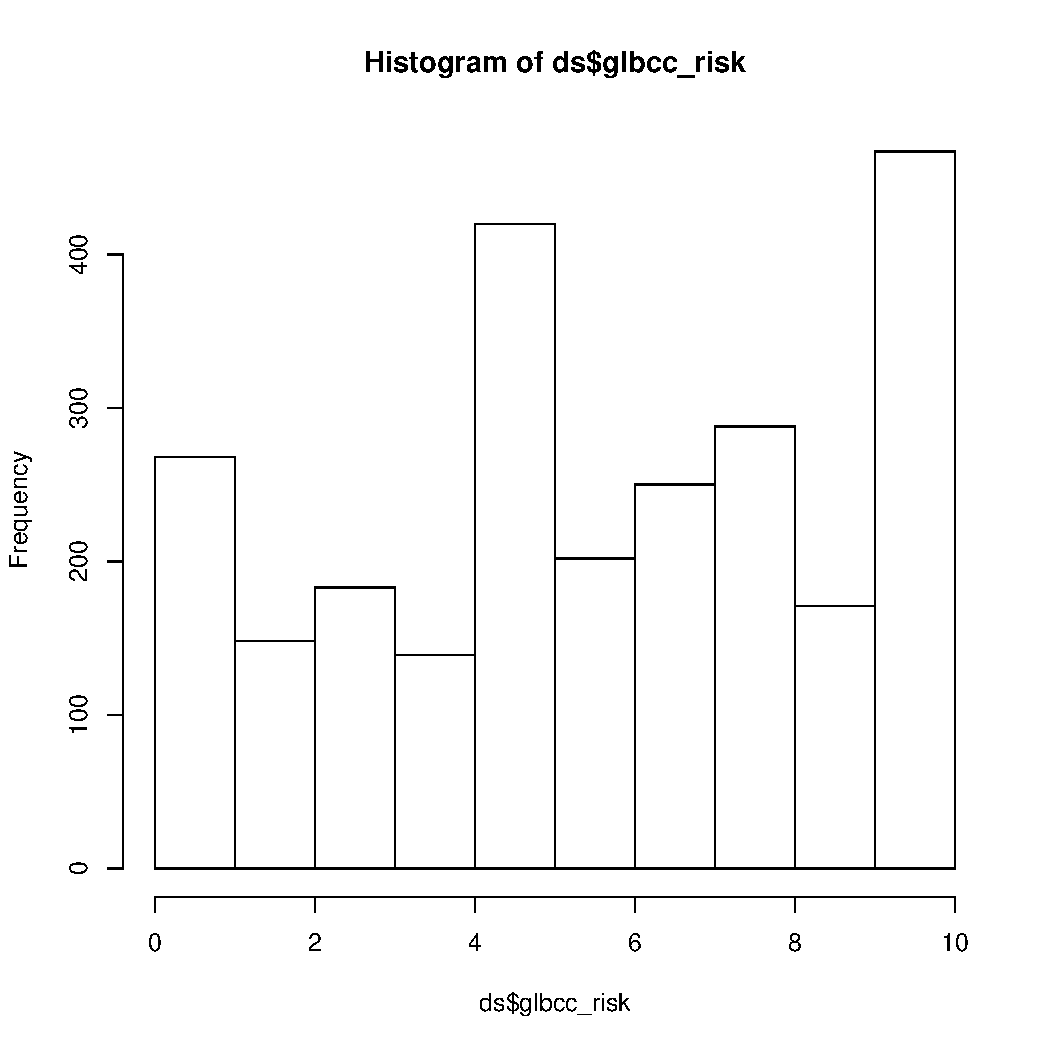
\includegraphics[width=\textwidth]{../03_Data/rskhist.pdf}%filename
                \caption{Histogram}
        \end{subfigure}
        \begin{subfigure}[b]{0.4\textwidth}
                \centering
                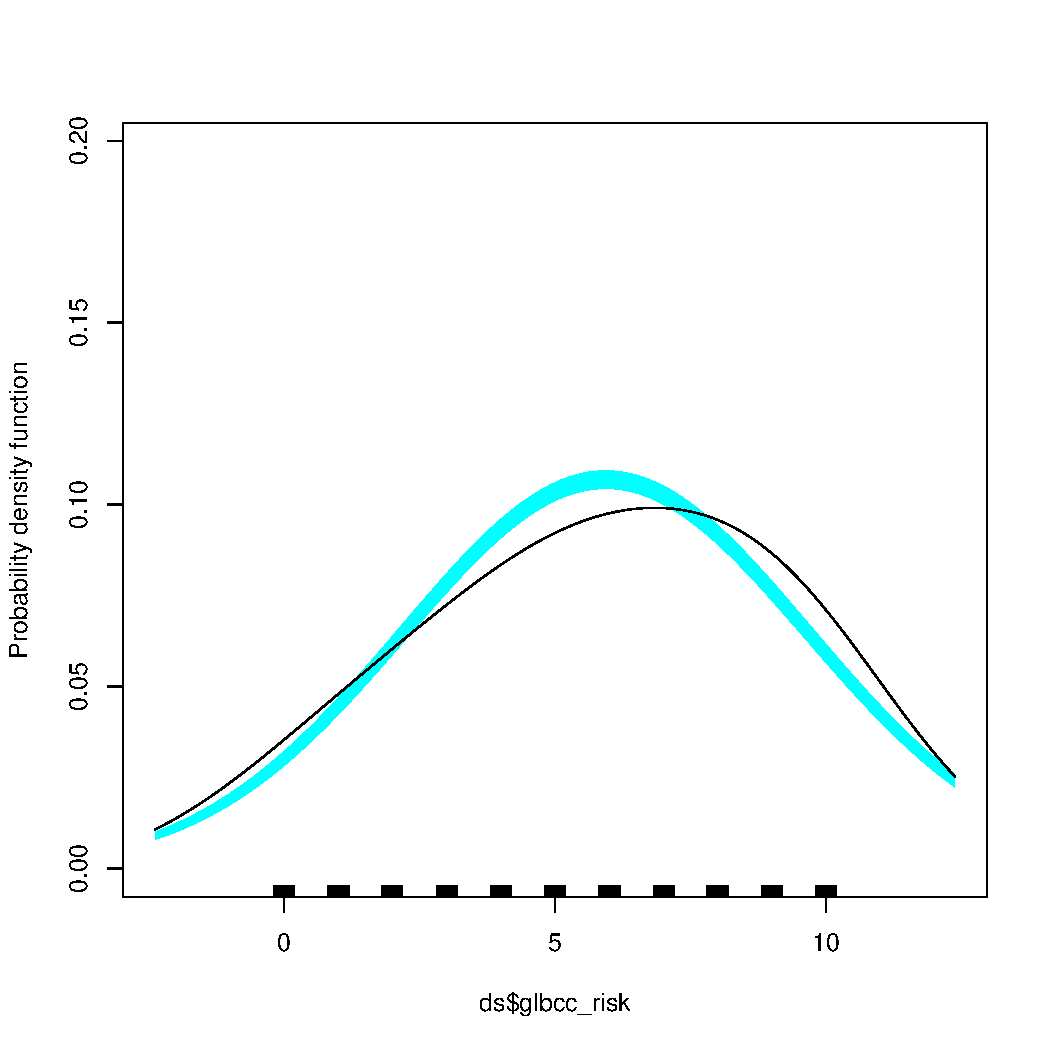
\includegraphics[width=\textwidth]{../03_Data/rskden.pdf}%filename
                \caption{Density Curve}
        \end{subfigure}
                \caption{Distribution of Age 
                \label{fig:rsk_2}} 
                                        
\end{figure}

You can also get an overview of your data using a table known as a frequency distribution. The frequency distribution summarizes how often each value of your variable occurs in the dataset.  If your variable has a limited number of values that it can take on, you can report all values, but if it has a large number of possible values (e.g., age of respondent), then you will want to create categories, or bins, to report those frequencies. In such cases, it is generally easier to make sense of the percentage distribution.  Table \ref{tab:ideology} is a frequency distribution for the ideology variable.  From that table we see, for example, that about one-third of all respondents are moderates. We see the numbers decrease as we move away from that category, but not uniformly.  There are a few more people on the conservative extreme than on the liberal side and that the number of people placing themselves in the penultimate categories on either end is greater than those towards the middle.  The histogram and density curve would, of course, show the same pattern.

The other thing to watch for here (or in the charts) is whether there is an unusual observation.  If one person scored 17 in this table, you could be pretty sure a coding error was made somewhere.  You cannot find all your errors this way, but you can find some, including the ones that have the potential to most seriously adversely affect your analysis.
  
\begin{table}[h]
\caption{Frequency Distribution for Ideology}
\label{tab:ideology}
\begin{tabular}{|l|c|c|c|}
\hline
Ideology & Frequency & Percentage & \begin{tabular}[c]{@{}c@{}}Cumulative \\ Percentage\end{tabular} \\ \hline
1 Strongly Liberal & 122 & 4.8 & 4.8 \\ \hline
2 & 279 & 11.1 & 15.9 \\ \hline
3 & 185 & 7.3 & 23.2 \\ \hline
4 & 571 & 22.6 & 45.8 \\ \hline
5 & 328 & 13.0 & 58.8 \\ \hline
6 & 688 & 27.3 & 86.1 \\ \hline
7 Strongly Conservative & 351 & 13.9 & 100.0 \\ \hline
Total & 2524 & 100 &  \\ \hline
\end{tabular}
\end{table}

\noindent In R, we can obtain the data for the above table with the following functions:

\begin{knitrout}
\definecolor{shadecolor}{rgb}{0.969, 0.969, 0.969}\color{fgcolor}\begin{kframe}
\begin{alltt}
\hlcom{# frequency counts for each level}
\hlkwd{table}\hlstd{(ds}\hlopt{$}\hlstd{ideol)}
\end{alltt}
\begin{verbatim}
## 
##   1   2   3   4   5   6   7 
## 122 279 185 571 328 688 351
\end{verbatim}
\begin{alltt}
\hlcom{# To view percentages}
\hlkwd{library}\hlstd{(dplyr)}
\hlkwd{table}\hlstd{(ds}\hlopt{$}\hlstd{ideol)} \hlopt \hlkwd{prop.table}\hlstd{()}
\end{alltt}
\begin{verbatim}
## 
##          1          2          3          4          5          6 
## 0.04833597 0.11053883 0.07329635 0.22622821 0.12995246 0.27258320 
##          7 
## 0.13906498
\end{verbatim}
\begin{alltt}
\hlcom{# multiply the numbers by 100 }
\hlkwd{table}\hlstd{(ds}\hlopt{$}\hlstd{ideol)} \hlopt \hlkwd{prop.table}\hlstd{()} \hlopt{*} \hlnum{100}
\end{alltt}
\begin{verbatim}
## 
##         1         2         3         4         5         6         7 
##  4.833597 11.053883  7.329635 22.622821 12.995246 27.258320 13.906498
\end{verbatim}
\end{kframe}
\end{knitrout}


Having obtained a sample, it is important to be able to characterize that sample.  In particular, it is important to understand the probability distributions associated with each variable in the sample. 

\subsection{Central Tendency} 
Measures of central tendency are useful because a single statistic can  be used to describe the distribution. We focus on three measures of central
tendency; the mean, the median, and the mode.  

\begin{grbox}
 \greybox{\textbf{Measures of Central Tendency}
   \begin{itemize}
   \item The Mean: The arithmetic average of the values
   \item The Median: The value at the center of the distribution 
   \item The Mode: The most frequently occurring value  
   \end{itemize}}   
\end{grbox}

We will primarily rely on the mean, because of its efficient property of representing the data. But medians -- particularly when used in conjunction with the mean - can tell us a great deal about the shape of the distribution of our data. We will return to this point shortly.

\subsection{Level of Measurement and Central Tendency}

The three measures of central tendency --  the mean, median, and mode -- each tell us something different about our data, but each has some limitations (especially when used alone). Knowing the mode tells us what is most common, but we do not know how common and, using it alone, would not even leave us confident that it is an indicator of anything very \textit{central}. When rolling in your data, it is generally a good idea to roll in all the descriptive  statistics that you can to get a good feel for them.

One issue, though, is that your ability to use a statistic is dependent on the level of measurement for the variable.  The mean requires you to add all your observations together. But you cannot perform mathematical functions on ordinal or nominal level measures. Your data must be measured at the interval level to calculate a meaningful mean. (If you ask R to calculate the mean student id number, it will, but what you get will be nonsense.) Finding the middle item in an order listing of your observations (the median) requires the ability to order your data, so your level of measurement must be at least ordinal. Therefore, if you have nominal level data, you can only report the mode (but no median or mean) so it is critical that you also look beyond central tendency to the overall distribution of the data.

\subsection{Moments} 

In addition to measures of central tendency,``moments" are important ways to characterize the shape of the distribution of a sample variable. Moments are applicable when the data measured is interval type (the level of measurement). The first four moments are those that are most often used.  

\begin{grbox}
\greybox{\textbf{The First Four Moments}
\begin{enumerate}
\item \textit{Expected Value}: The expected value of a variable, $E(X)$ is its mean. 
\begin{center}
$E(X) = \bar{X}=\frac{\sum X_{i}}{n}$
\end{center}
\item \textit{Variance}: The variance of a variable concerns the way that the observed \\  
values are spread around either side of the mean. 
  \begin{center}
 $s^{2}_{x}=\frac{\sum (X-\bar{X})^{2}}{(n-1)}$   
  \end{center}
\item \textit{Skewness}: The skewness of a variable is a measure of its
  asymmetry. 
  \begin{center}
    $S = \frac{\sum (X-\bar{X})^{3}}{(n-1)}$
  \end{center}
\item \textit{Kurtosis}: The kurtosis of a variable is a measure of its
peakedness. 
  \begin{center}
    $K = \frac{\sum (X-\bar{X})^{4}}{(n-1)}$
  \end{center}
\end{enumerate}}  
\end{grbox}

\subsection{First Moment -- Expected Value}

The {\textit{expected value} of a variable is the value you would obtain if you could multiply all possible values within a population by their probability of occurrence. Alternatively, it can be understood as the mean value for a population variable. An expected value is a theoretical number , because we usually cannot observe all possible occurrences of a variable. The mean value for a sample is the average value for the variable $X$, and is calculated by adding the values of $X$ and dividing by the sample size $n$:  
\begin{equation} 
\bar{X} = \frac{(x_{1}+x_{2}+x_{3}+x_{n})}{n}
\end{equation} 
This can be more compactly expressed as:
\begin{equation}
\bar{X}=\frac{\sum X_{i}}{n}  
\end{equation}
The mean of a variable can be calculated in \texttt{R} using the \texttt{mean} function. Here we illustrate the calculation of means for our measures of \texttt{ideology}, \texttt{age}, and \texttt{perceived risk of climate change}\footnote{The ``na.rm=TRUE" portion of the following code simply tells R to exclude the missing (NA) values from calculation}.

\begin{knitrout}
\definecolor{shadecolor}{rgb}{0.969, 0.969, 0.969}\color{fgcolor}\begin{kframe}
\begin{alltt}
\hlkwd{mean}\hlstd{(ds}\hlopt{$}\hlstd{ideol,} \hlkwc{na.rm}\hlstd{=}\hlnum{TRUE}\hlstd{)}
\end{alltt}
\begin{verbatim}
## [1] 4.652932
\end{verbatim}
\begin{alltt}
\hlkwd{mean}\hlstd{(ds}\hlopt{$}\hlstd{age,} \hlkwc{na.rm}\hlstd{=}\hlnum{TRUE}\hlstd{)}
\end{alltt}
\begin{verbatim}
## [1] 60.36749
\end{verbatim}
\begin{alltt}
\hlkwd{mean}\hlstd{(ds}\hlopt{$}\hlstd{glbcc_risk,} \hlkwc{na.rm}\hlstd{=}\hlnum{TRUE}\hlstd{)}
\end{alltt}
\begin{verbatim}
## [1] 5.945978
\end{verbatim}
\end{kframe}
\end{knitrout}
 
\subsection{The Second Moment -- Variance and Standard Deviation}

The \textit{variance} of variable is a measure that illustrates how a variable is spread, or distributed, around its mean. For samples, it is expressed as:  
\begin{equation}
s^{2}_{x}=\frac{\sum (X-\bar{X})^{2}}{(n-1)}  
\end{equation}
The population variance is expressed as: $\sigma^{2}_{X}$. 

Variance is measured in \texttt{squared} deviations from the mean, and the sum of these squared variations is termed the \textbf{total sum of squares}. Why squared deviations? Why not just sum the differences? While the latter strategy would seemingly be simpler, but it would always sum to zero. By squaring the deviations we make them all positive, so the sum of squares will always be a positive number.

\begin{description}
\item[Total Sum of Squares] Is the squared summed total of the variation of a variable around its mean
\end{description}
This can be expressed as: 
\begin{equation}
TSS_{x} = \sum(X_{i}-\bar{X})^{2}   
\end{equation}
therefore; 
\begin{equation}
s^{2}_{x} = \frac{TSS_{x}}{(n-1)}  
\end{equation}

The square root of variance, $\sigma^{2}_{x}$, is the \textit{standard deviation} (s.d.) of a variable, $\sigma_{x}$. The sample s.d. is expressed as: 
\begin{equation}
s_{x} = \sqrt{\frac{\sum(X-\bar{X})^{2}}{(n-1)}}  
\end{equation}
This can also be expressed as $\sqrt{s^2_{x}}$.  The standard deviation of a variable can be obtained in \texttt{R} with the \texttt{sd} function.\footnote{What's with those (n-1) terms in the denominators? These represent the ``degrees of freedom" we have to calculate the average squared deviations and variance. We ``use up" one of our observations to be able to calculate the first deviation -- because without that first observation, what would there be to deviate from?}

\begin{knitrout}
\definecolor{shadecolor}{rgb}{0.969, 0.969, 0.969}\color{fgcolor}\begin{kframe}
\begin{alltt}
\hlkwd{sd}\hlstd{(ds}\hlopt{$}\hlstd{ideol,} \hlkwc{na.rm}\hlstd{=}\hlnum{TRUE}\hlstd{)}
\end{alltt}
\begin{verbatim}
## [1] 1.731246
\end{verbatim}
\begin{alltt}
\hlkwd{sd}\hlstd{(ds}\hlopt{$}\hlstd{age,} \hlkwc{na.rm}\hlstd{=}\hlnum{TRUE}\hlstd{)}
\end{alltt}
\begin{verbatim}
## [1] 14.20894
\end{verbatim}
\begin{alltt}
\hlkwd{sd}\hlstd{(ds}\hlopt{$}\hlstd{glbcc_risk,} \hlkwc{na.rm}\hlstd{=}\hlnum{TRUE}\hlstd{)}
\end{alltt}
\begin{verbatim}
## [1] 3.071251
\end{verbatim}
\end{kframe}
\end{knitrout}

\subsection{The Third Moment -- Skewness}

\textit{Skewness} is a measure of the asymmetry of a distribution. It is based on the
third moment and is expressed as: 
\begin{equation}
\frac{\sum (X-\bar{X})^{3}}{(n-1)}  
\end{equation}
Skewness is calculated by dividing the third moment by the the cube of
the s.d. 
\begin{equation}
S = \frac{\frac{\sum (X-\bar{X})^{3}}{(n-1)}}{(\sqrt{\frac{\sum
    (X-\bar{X})^{2}}{(n-1)})^{3}}}    
\end{equation}
Specifically, skewness refers to the position of the expected value (i.e., mean) of a variable distribution relative to its median. When the mean and median of a variable are roughly equal, $\bar{Y} \approx Md_{Y}$, then the distribution is considered approximately symmetrical, $S = 0$. This means that an equal proportion of the distribution of the variable lies on either side of the mean. However, when the mean is larger than the median,
$\bar{Y} > Md_{Y}$, then the distribution has a \textit{positive} skew, $S > 0$. When the median is larger than the mean, $\bar{Y} < Md_{Y}$, this is a \textit{negative} skew, $S < 0$. This is illustrated in Figure \ref{fig:disshape}. Note that for a normal distribution, $S=0$. 
      
\begin{figure}
  \centering
  \includegraphics[width=4in]%
    {../03_Data/distroshapes.pdf}% picture filename
  \caption{Distributional Shapes \label{fig:disshape}}
\end{figure}

\subsection{The Fourth Moment -- Kurtosis}

The \textit{kurtosis} of a distribution refers to the the peak of a variable (i.e., the mode) and the relative frequency of observations in the tails. It is based on the fourth moment which is expressed as: 
\begin{equation}
\frac{\sum (X-\bar{X})^{4}}{(n-1)}  
\end{equation}
Kurtosis is calculated by dividing the fourth moment by the square of the second moment (i.e., variance). 
\begin{equation}
 K =  \frac{\frac{\sum (X-\bar{X})^{4}}{(n-1)}}{(\frac{\sum (X-\bar{X})^{2}}{(n-1)})^{2}} 
\end{equation}
In general, higher kurtosis is indicative of a distribution where the variance is a result of low frequency yet more extreme observed values. In addition, when $K < 3$, the distribution is \textit{platykurtic}, which is flatter and/or more "short-tailed" than a normal distribution. When $K > 3$ the distribution is \textit{leptokurtic}, which is a slim, high peak and long tails. In a normal distribution $K=3$. 
 
\subsection{Order Statistics}

Apart from central tendency and moments, probability distributions can also be characterized by \textbf{order statistics}. Order statistics are based on the position of a value in an ordered list. Typically, the list is ordered from low values to high values.


\begin{grbox}
\greybox {\textbf{Order Statistics} 

Summaries of values based on position in an ordered list of all values.  Types of order statistics include the minimum value, the maximum value, the median, quartiles, and percentiles. 
  \begin{itemize}
  \item \textit{Minimum Value}: The lowest value of a distribution 
\item \textit{Maximum Value}: The highest value of a distribution
\item \textit{Median}: The value at the center of a distribution
\item \textit{Quartiles}: Divides the values into quarters 
\item \textit{Percentiles}: Divides the values into hundredths 
  \end{itemize}}
\end{grbox}

\subsubsection{Median}

The \textit{median} is the value at the center of the distribution, therefore 50\% of the observations in the distribution will have values above
the median and 50\% will have values below. For samples with a $n$-size that is an odd number, the median is simply the value in the middle. For example, with a sample consisting of the observed values of $1, 2, 3, 4, 5$, the median is $3$. Distributions with an even numbered $n$-size, the median is the average of the two middle values. The median of a sample consisting of the observed values of $1, 2, 3, 4, 5, 6$
would be $\frac{3+4}{2}$ or 3.5. 

The the median is the order statistic for central tendency. In addition, it is more ``robust'' in terms of extreme values than the mean. Extremely high values in a distribution can pull the mean higher, and extremely low values pull the mean lower. The median is less sensitive to these extreme values. The median is therefore the basis for ``robust estimators," to be discussed later in this book.

\subsubsection{Quartiles}

\textit{Quartiles} split the observations in a distribution into quarters. The first quartile, $Q1$, consists of observations whose values are within
the first 25\% of the distribution. The values of the second quartile, $Q2$, are contained within the first half (50\%) of the distribution, and is marked by the distribution's median. The third quartile, $Q3$, includes the first 75\% of the observations in the distribution.  

The interquartile range (IQR) measures the spread of the ordered values. It is calculated by subtracting $Q1$ from $Q3$.
\begin{equation}
 IQR = Q_{3}-Q_{1}  
\end{equation}
The IQR contains the middle 50\% of the distribution. 

We can visually examine the order statistics of a variable with a boxplot. A boxplot displays the range of the data, the first and third quartile, the median, and any outliers. To obtain a boxplot use the \texttt{boxplot} command. It is shown in Figure \ref{fig:boxrsk}. 

\begin{knitrout}
\definecolor{shadecolor}{rgb}{0.969, 0.969, 0.969}\color{fgcolor}\begin{kframe}
\begin{alltt}
\hlkwd{ggplot}\hlstd{(ds,} \hlkwd{aes}\hlstd{(}\hlstr{""}\hlstd{, glbcc_risk))} \hlopt{+}
  \hlkwd{geom_boxplot}\hlstd{()}
\end{alltt}
\end{kframe}
\end{knitrout}

\begin{figure}
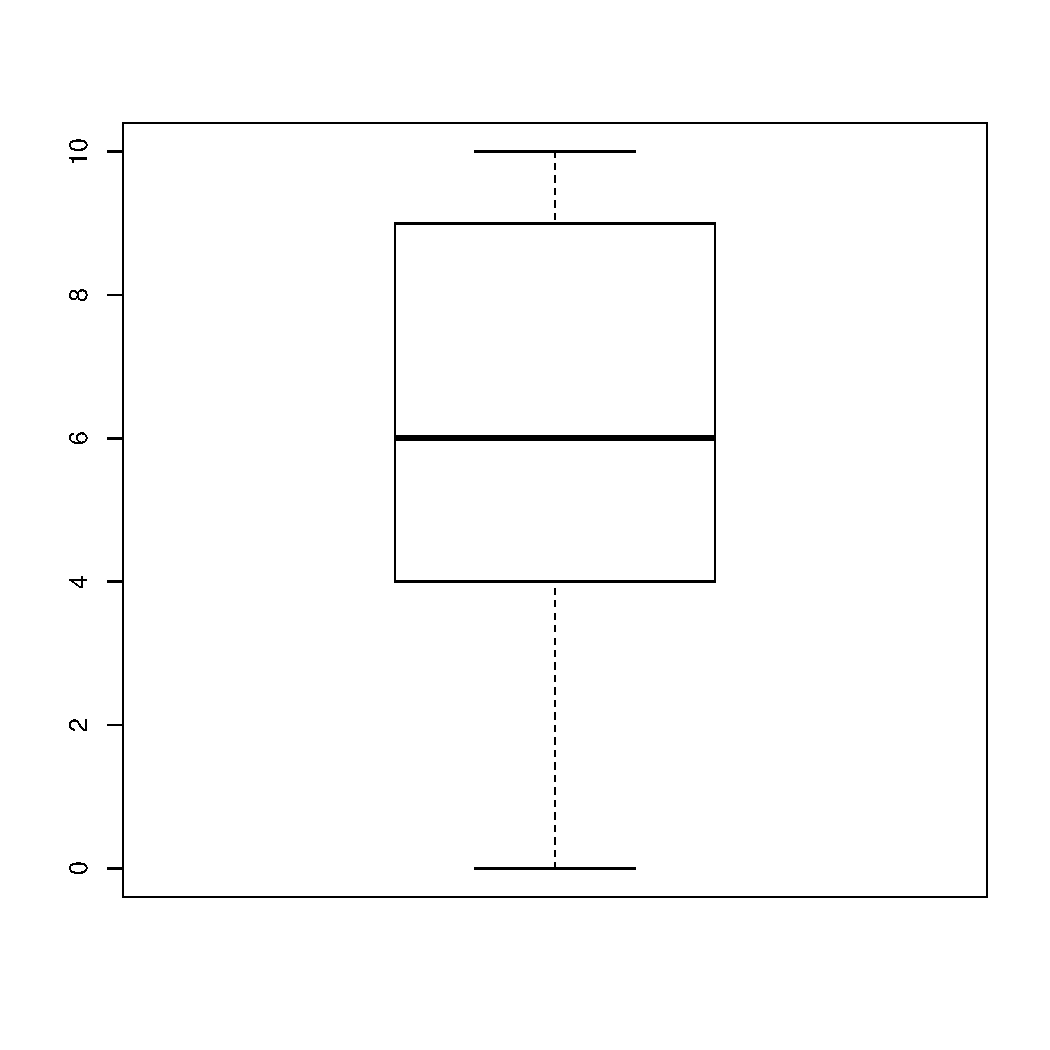
\includegraphics[width=4in]{../03_Data/gccrskbox.pdf}%filname
\caption{Box-plot of Climate Change Risk 
\label{fig:boxrsk}}
\end{figure} 

\subsubsection{Percentiles}

\textit{Percentiles} list the data in hundredths. For example, scoring in the 99th percentile on the GRE means that 99\% of the other test takers
had a lower score. Percentiles can be incorporated with quartiles (and/or other order statistics) such that:
\begin{itemize}
\item First Quartile: 25th percentile 
\item Second Quartile: 50th percentile (the median) 
\item Third Quartile: 75th percentile 
\end{itemize}

Another way to compare a variable distribution to a theoretical distribution is with a quantile-comparison plot (qq plot). A qq plot displays the observed percentiles against those that would be expected in a normal distribution. This plot is often useful for examining the tails of the distribution, and deviations of a distribution from normality. This is shown in Figure \ref{fig:qqrsk}. 

\begin{knitrout}
\definecolor{shadecolor}{rgb}{0.969, 0.969, 0.969}\color{fgcolor}\begin{kframe}
\begin{alltt}
\hlkwd{ggplot}\hlstd{(ds,} \hlkwd{aes}\hlstd{(}\hlkwc{sample} \hlstd{= glbcc_risk))} \hlopt{+}
  \hlkwd{stat_qq}\hlstd{()}
\hlkwd{dev.off}\hlstd{()}
\end{alltt}
\end{kframe}
\end{knitrout}

\begin{figure}[!htp]
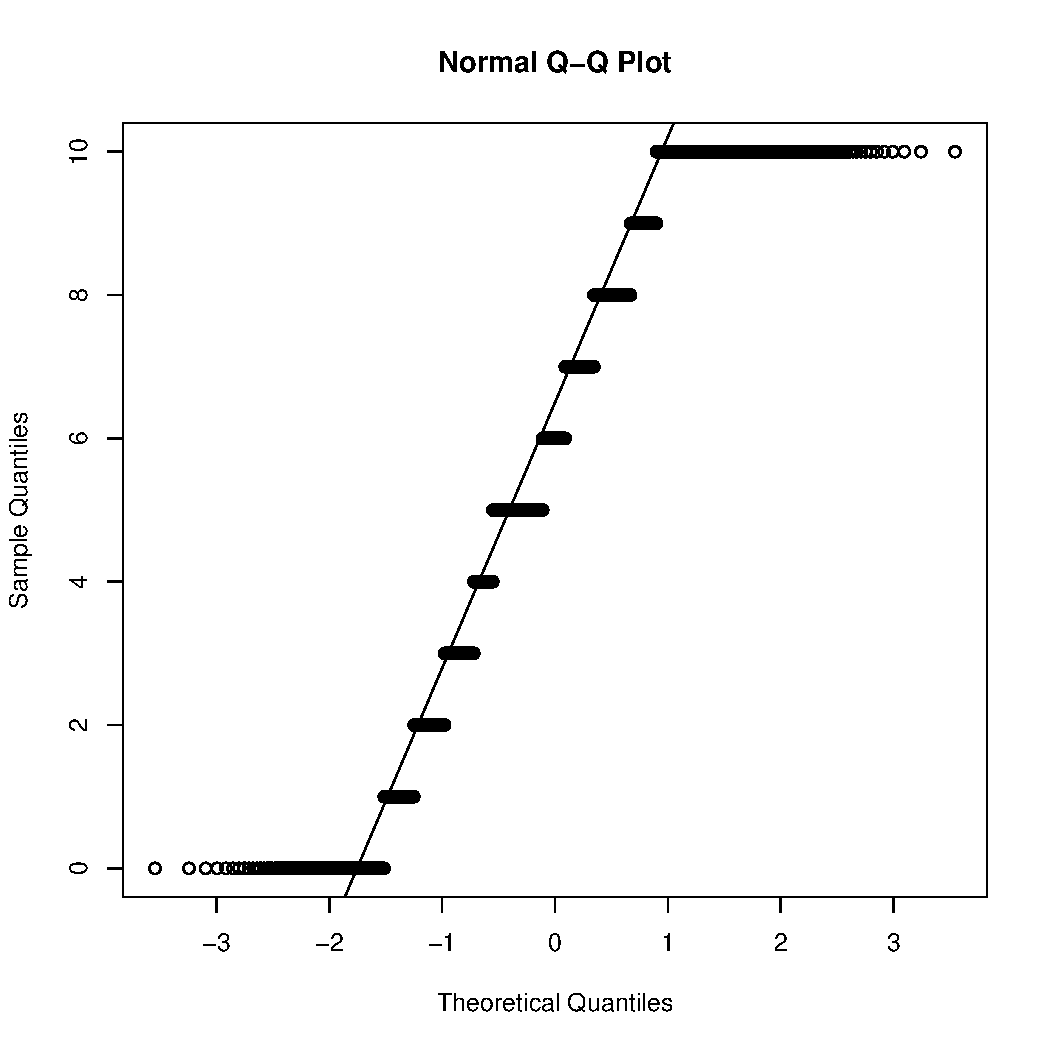
\includegraphics[width=4in]{../03_Data/gccrskqq.pdf}%filename
\caption{QQ Plot of Climate Change Risk 
\label{fig:qqrsk}}
\end{figure}    

The qq plot provides an easy way to observe departures of a distribution from normality. For example, the plot shown in Figure \ref{fig:qqrsk} indicates the perceived risk measure has more observations in the tails of the distribution than would be expected if the variable was normally distributed.

\texttt{R} provides several ways to examine the central tendency, moments, and order statistics for variables and for entire data sets.  The \texttt{summary} function produces the minimum value, the first quartile, median, mean, third quartile, max value, and the number of missing values (Na's).

\begin{knitrout}
\definecolor{shadecolor}{rgb}{0.969, 0.969, 0.969}\color{fgcolor}\begin{kframe}
\begin{alltt}
\hlkwd{summary}\hlstd{(ds}\hlopt{$}\hlstd{ideol,} \hlkwc{na.rm}\hlstd{=}\hlnum{TRUE}\hlstd{)}
\end{alltt}
\begin{verbatim}
##    Min. 1st Qu.  Median    Mean 3rd Qu.    Max.    NA's 
##   1.000   4.000   5.000   4.653   6.000   7.000      23
\end{verbatim}
\begin{alltt}
\hlkwd{summary}\hlstd{(ds}\hlopt{$}\hlstd{age,} \hlkwc{na.rm}\hlstd{=}\hlnum{TRUE}\hlstd{)}
\end{alltt}
\begin{verbatim}
##    Min. 1st Qu.  Median    Mean 3rd Qu.    Max. 
##   18.00   52.00   62.00   60.37   70.00   99.00
\end{verbatim}
\begin{alltt}
\hlkwd{summary}\hlstd{(ds}\hlopt{$}\hlstd{gcclb_risk,} \hlkwc{na.rm}\hlstd{=}\hlnum{TRUE}\hlstd{)}
\end{alltt}
\begin{verbatim}
## Length  Class   Mode 
##      0   NULL   NULL
\end{verbatim}
\end{kframe}
\end{knitrout}
 
We can also use the \texttt{describe} function in the \texttt{psych} package to obtain more descriptive statistics, including skewness and
kurtosis. 

\begin{knitrout}
\definecolor{shadecolor}{rgb}{0.969, 0.969, 0.969}\color{fgcolor}\begin{kframe}
\begin{alltt}
\hlkwd{library}\hlstd{(psych)}
\hlkwd{describe}\hlstd{(ds}\hlopt{$}\hlstd{ideol)}
\end{alltt}
\begin{verbatim}
##    vars    n mean   sd median trimmed  mad min max range  skew kurtosis
## X1    1 2524 4.65 1.73      5    4.75 1.48   1   7     6 -0.45     -0.8
##      se
## X1 0.03
\end{verbatim}
\end{kframe}
\end{knitrout}
 
\subsection{Summary}
 
It is a serious mistake to get into your data analysis without understanding the basics of your data.  Knowing their range, the general distribution of your data, the shape of that distribution, their central tendency, and so forth will give you important clues as you move through your analysis and interpretation and prevent serious errors from occurring.  Readers also often need to know this information to provide a critical review of your work. 
 
Overall, this chapter has focused on understanding and characterizing data. We refer to the early process of evaluating a data set as rolling in the data -- getting to know the characteristic shapes of the distributions of each of the variables, the meanings of the scales, and the quality of the observations.  The discussion of central tendency, moments, and order statistics are all tools that you can use for that purpose. As a practicing scholar, policy analyst or public administration practitioner, this early stage in quantitative analysis is not optional; a failure to carefully and thoroughly understand your data can result in analytical disaster, excruciating embarrassment, and maybe even horrible encounters with the Killer Rabbit of Caerbannog. 
 
Think of rolling in the data, then, as your version of the Holy Hand Grenade of Antioch.
\end{document}
